% !TEX root = results_only.tex

\section{Results}

describe the results generally

\subsection{Control case - uniform risk on a uniform population}

% latex table generated in R 3.4.0 by xtable 1.8-2 package
% Sat Aug  5 20:02:24 2017
\begin{table}[ht]
\centering
\begin{tabular}{lrrr}
  \hline
 & Oracle & Silverman & CV \\ 
  \hline
MISE & 0.000012 & 0.000013 & 0.000013 \\ 
  Relative MISE & 0.117027 & 0.127810 & 0.127803 \\ 
  MIAE & 0.002801 & 0.002922 & 0.002922 \\ 
  Relative MIAE & 0.280127 & 0.292163 & 0.292156 \\ 
  Max Error & 0.008572 & 0.009040 & 0.009040 \\ 
  Peak bias & 0.003361 & 0.005616 & 0.005615 \\ 
  Relative Peak bias & 0.336092 & 0.561583 & 0.561492 \\ 
  Peak drift & 5.163912 & 5.190480 & 5.190393 \\ 
  Relative Peak drift & 0.737702 & 0.741497 & 0.741485 \\ 
  Centroid bias & 0.002819 & 0.003733 & 0.003733 \\ 
  Relative Centroid bias & 0.281890 & 0.373345 & 0.373340 \\ 
  Centroid drift & 5.093476 & 5.086491 & 5.086412 \\ 
  Relative Centroid drift & 0.727639 & 0.726642 & 0.726630 \\ 
   \hline
\end{tabular}
\caption{Mean error rates} 
\label{tbl:mean_error_rates}
\end{table}


\begin{figure}[tb]
    \centering
    \begin{subfigure}[t]{0.45\textwidth}
    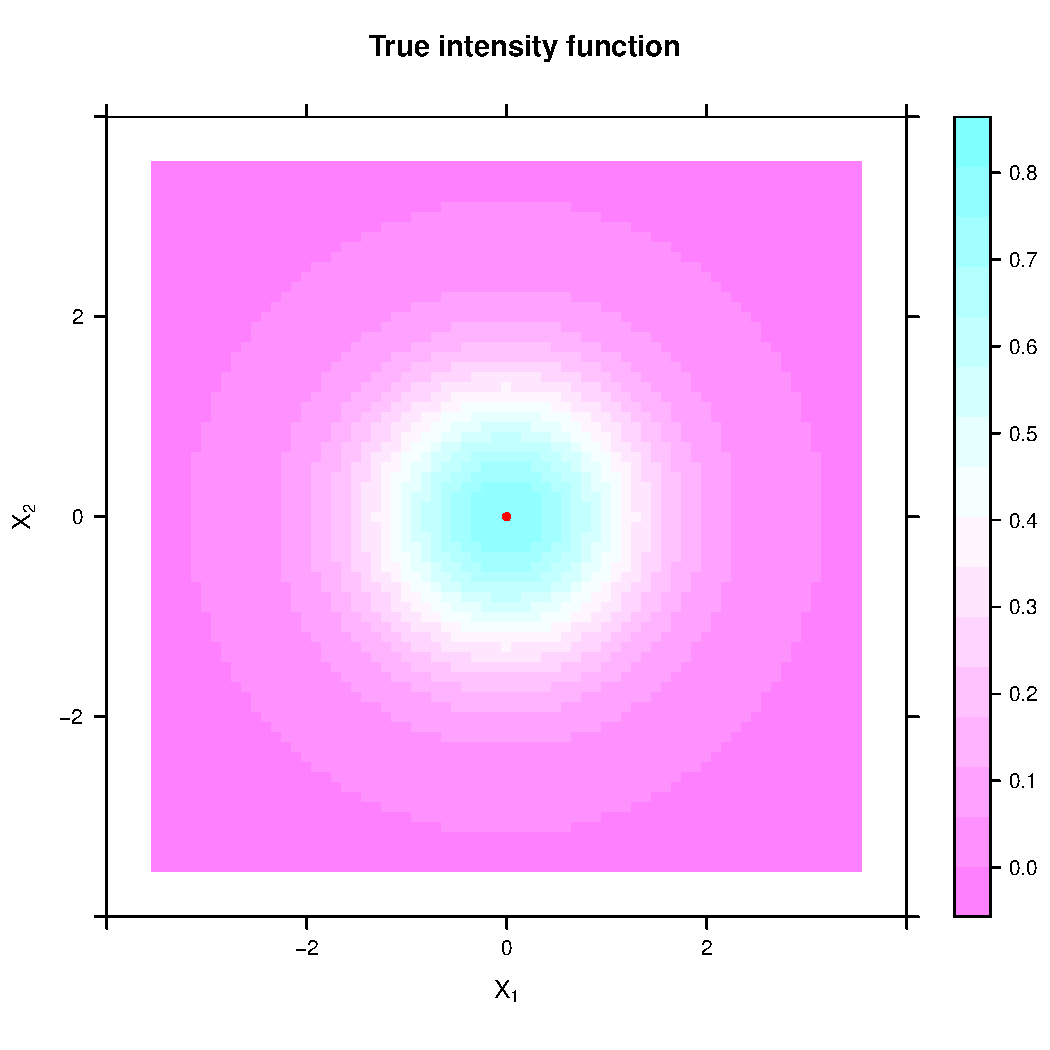
\includegraphics[width=\textwidth]{results/unif_100_1_unif/output/true_intensity_heatmap}
    \caption{True intensity}
    \end{subfigure}
    \begin{subfigure}[t]{0.45\textwidth}
    \includegraphics[width=\textwidth]{results/unif_100_1_unif/output/oracle_intensity_heatmap}
    \caption{Oracle estimate}
    \end{subfigure}
    \begin{subfigure}[b]{0.45\textwidth}
    \includegraphics[width=\textwidth]{results/unif_100_1_unif/output/silverman_intensity_heatmap}
    \caption{Silverman estimate}
    \end{subfigure}
    \begin{subfigure}[b]{0.45\textwidth}
    \includegraphics[width=\textwidth]{results/unif_100_1_unif/output/CV_intensity_heatmap}
    \caption{Cross-validation estimate}
    \end{subfigure}
    \label{fig:cases_unif_100_unif}
    \caption{Example cases: uniform intensity on uniform population, 100 cases}
\end{figure}

\begin{figure}[tb]
    \centering
    \begin{subfigure}[b]{0.45\textwidth}
    \includegraphics[width=\textwidth]{results/unif_100_1_unif/output/ise-relative-histogram}
    \caption{Relative ISE}
    \end{subfigure}
    \begin{subfigure}[b]{0.45\textwidth}
    \includegraphics[width=\textwidth]{results/unif_100_1_unif/output/ise-histogram}
    \caption{Absolute ISE}
    \end{subfigure}
    \caption[ISE: uniform on uniform]{Integrated squared error histogram for uniform intensity on a uniform population, 100 cases}
    \label{fig:ise_unif_100_1_unif}
\end{figure}

\subsection{Single-peak risk on a uniform population}

\subsection{Varying the number of cases}

\subsection{Varying the size of the population}

\subsection{Varying the decay of the risk function}

\subsection{Varying the decay of the population density}

\subsection{Varying the number of peaks in the risk function}

\subsection{Varying the distance between peaks}

